\documentclass[11pt]{article}
\usepackage{eadca-template}
\usepackage[plain]{algorithm}

\usepackage[brazil,english]{babel}
\usepackage[utf8]{inputenc}
\usepackage[T1]{fontenc}

\usepackage{graphicx,url}
\usepackage[hang]{subfigure}
\usepackage{psfrag}

\usepackage[table]{xcolor}

\usepackage{booktabs}

\sloppy


\title{The Name of the Title is Hope}

\author{Caluã de Lacerda Pataca \and Paula Dornhofer Paro Costa}
\address{\email{\{calua.pataca@gmail.com,paulad@unicamp.br\}}}

\begin{document}

\hyphenation{}
\pagestyle{fancy}

%%%%%%%%%%%%%%%%%%%%%%%%%%%%%%%%%%%%%%%%%%%%%%%%%%%%%%%%%%%%%%%%%%%%%%%%%%%%%
\twocolumn[
\maketitle
\thispagestyle{fancy}
\selectlanguage{english}

   \begin{abstract}
   \end{abstract}

  \keywords{}

]
%%%%%%%%%%%%%%%%%%%%%%%%%%%%%%%%%%%%%%%%%%%%%%%%%%%%%%%%%%%%%%%%%%%%%%%%%%%%%
\selectlanguage{brazil}

  \section{Introdu\c{c}\~{a}o}
  \label{sec:introducao}

   .

  %%%%%%%%%%%%%%%%%%%%%%%%%%%%%%%%%%%%%%%%%%%%%%%%%%%%%%%%%%%%%%%%%%%%%%%%%%%%%
  \section{Abordagem}
  \label{sec:abordagem}
  
  Nossa abordagem tem duas frentes principais: (1) escolha e extração de {\itshape features} acústicas de uma dada enunciação sonora; (2) tratamento e representação dessas {\itshape features} enquanto modulações tipográficas na transcrição dessa mesma enunciação.
  
  Para a primeira, adotamos {\itshape features} prosódicas, ou seja, aquelas tipicamente relacionadas à propriedades expressivas no falar de sílabas, palavras ou frases, e que contemplam características como ritmo, intensidade, tom etc. Especificamente, escolhemos {\itshape raiz do valor quadrático médio} \textsc{(rms)}, como medida de intensidade, e {\itshape frequência fundamental} $(f_0)$ --- em ambos os casos, {\itshape features} que, se consideradas no nível da sílaba, retêm informações sobre expressividade afetiva da fala \cite{rao2010characterization}.
  
  Para a representação das {\itshape features}, optamos por usar a tecnologia {\itshape variable fonts}, introduzida pela especifação 1.8 da OpenType \cite{varfontssepcs} em 2016 e que, desde então, já está incorporada nos principais sistemas operacionais \cite{varfontossupport} e navegadores \cite{varfontbrowsersupport}. Nela, os pontos que compõe o contorno do desenho de cada glifo em uma determinada fonte podem ter suas coordenadas deslocadas a partir de diversos eixos de variação, combináveis entre si e que permitem, assim, que a aparência de cada letra seja modulada dinamicamente. O exemplo mais comum de um eixo de variação seria o de {\itshape peso}, que varia desde uma letra mais fina até uma mais grossa, tornando contínuas e combináveis as variações que tipicamente são discretas (e.g. uma fonte não-{\itshape variable} terá um arquivo para o negrito, outro para o regular, outro para o leve etc). Em nosso teste, usamos 4 modulações tipográficas. {\itshape Peso}, {\itshape largura}, {\itshape inclinação} e {\itshape baseline shift}, como ilustradas pela Figura~\ref{fig:type_modulations}.
  
\begin{figure}[H]
     {\centering
    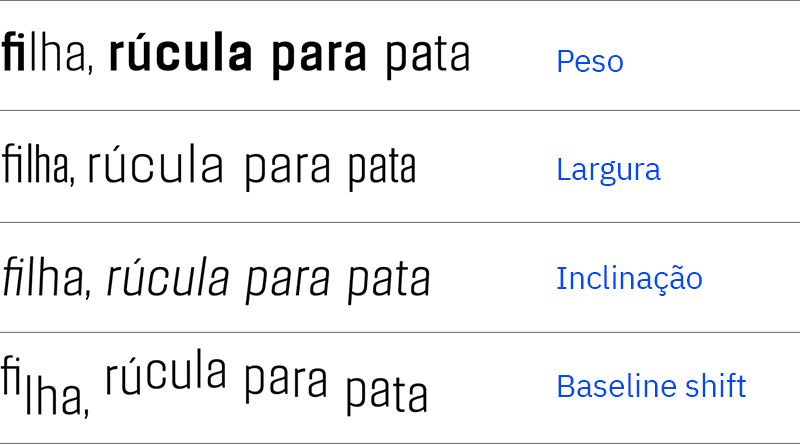
\includegraphics[width=\linewidth]{fig/modulacoes.png}
     \caption{As quatro modulações tipográficas avaliadas no experimento}
     \label{fig:type_modulations}\par}
\end{figure}
  
  \section{Metodologia}
  \label{sec:metodologia}
 
  


\section{Resultados}
  \label{sec:resultados}
  
  Na Tabela~\ref{tab:type_perf} apresentamos quão frequentemente cada modulação tipográfica (dada pela coluna) foi escolhida quando comparada às outras três modulações levando em conta cada emoção (dada pela linha) e cada {\itshape feature} sendo representada. Ressaltamos em verde as células que indicam a configuração preferida de modulação tipográfica e {\itshape feature} representada para uma dada emoção. Por exemplo, considerando a emoção {\itshape raiva}, a configuração com maior preferência pelos participantes foi {\itshape peso} representando $f_0$.
  
\begin{table}
    \begin{tabular*}{\linewidth}{lcccc}
        \toprule
        \multicolumn{5}{c}{ \textbf{\textsc{rms} enquanto {\itshape feature} representada} }     \\
        \midrule
        emoção & peso & largura & inclinação & baseline shift  \\
        \midrule
        raivosa       & 83\% & 34\% & 43\% & 39\% \\
        alegre        & 34\% & 54\% & 47\% & 64\% \\
        neutra        & 47\% & 52\% & \cellcolor[HTML]{9ef7cd}76\% & 25\% \\
        triste        & 45\% & 52\% & 46\% & 58\% \\
        surpresa      & \cellcolor[HTML]{9ef7cd}72\% & 38\% & 49\% & 43\% \\
        \midrule
        \multicolumn{5}{c}{ \textbf{$f_0$ enquanto {\itshape feature} representada} }      \\
        \midrule
        emoção & peso & largura & inclinação & baseline shift  \\
        \midrule
        raivosa       & \cellcolor[HTML]{9ef7cd}87\% & 46\% & 45\% & 26\% \\
        alegre        & 28\% & 66\% & 40\% & \cellcolor[HTML]{9ef7cd}69\% \\
        neutra        & 47\% & 55\% & 63\% & 35\% \\
        triste        & 21\% & 57\% & 39\% & \cellcolor[HTML]{9ef7cd}79\% \\
        surpresa      & 71\% & 43\% & 41\% & 44\% \\
        \bottomrule
    \end{tabular*}
    \caption{Preferência dos participantes para cada uma das modulações tipográficas por emoção por {\itshape feature}. }
    \label{tab:type_perf}
\end{table}
  
  Nas Figuras~\ref{fig:font_weight_as_f0} e \ref{fig:baseline_shift_as_f0}, mostramos como a performance das modulações tipográficas de {\itshape peso} e {\itshape baseline shift}, quando usadas para representar $f_0$, se correlacionam à média da distância entre o {\itshape centróide} e a $f_0$ em cada frase. Essa é uma métrica de intensidade mais robusta que \textsc{rms}, pois parte da constatação de que uma voz enunciada com maior intensidade tende a ter uma centróide de frequência mais elevada sem um aumento proporcional $f_0$. Assim, é pouco sensível a pequenas inconsistências no ambiente de gravação, como a distância entre a atriz e o microfone, ao contrário do \textsc{rms}.
  
  Na Figura~\ref{fig:font_weight_as_f0}, plotamos a performance da modulação tipográfico {\itshape peso} quando usada para representar $f_0$ --- nas duas frases, a equação de regressão foi significante, com ``filha'' apresentando um $R^2$ de .93 e performance esperada de $(C-f_0) * 10^{-3} - 1.29$ e ``passarinho'' um $R^2$ de .89. e performance esperada de $(C-f_0) * 10^{-3} - 2.61$. Na Figura~\ref{fig:baseline_shift_as_f0}, performance de {\itshape baseline shift} representando $f_0$ --- nesse caso, a equação de regressão não foi significante, motivo pelo qual é apresentada como linha tracejada no gráfico.
  
\begin{figure}[H]
     {\centering
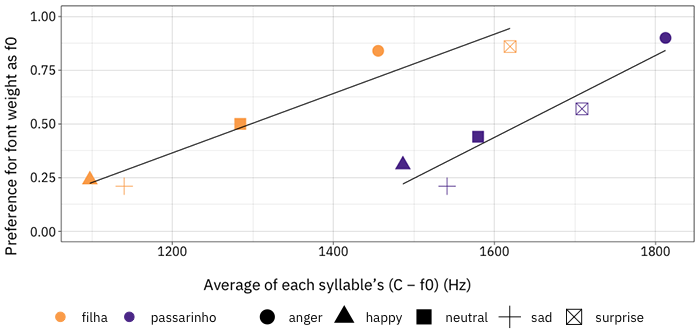
\includegraphics[width=\linewidth]{fig/font_weight_as_pitch.png}
     \caption{Performance de {\itshape Peso} como representação de $f_0$}
     \label{fig:font_weight_as_f0}\par}
\end{figure}

\begin{figure}[H]
     {\centering
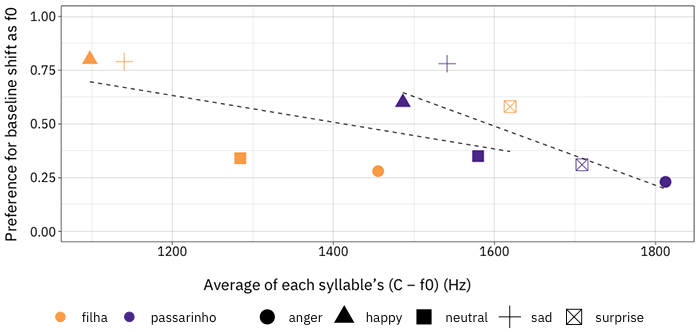
\includegraphics[width=\linewidth]{fig/baseline_shift_as_pitch.png}
     \caption{Performance de {\itshape baseline shift} como representação de $f_0$}
     \label{fig:baseline_shift_as_f0}\par}
\end{figure}

\section{Conclus\~{o}es}
  \label{sec:conclusoes}

%%%%%%%%%%%%%%%%%%%%%%%%%%%%%%%%%%%%%%%%%%%%%%%%%%%%%%%%%%%%%%%%%%%%%%%%%%%%%
  \bibliographystyle{plain}

   \bibliography{bib-template}

\end{document}
